\documentclass[]{spie}  %>>> use for US letter paper
%\documentclass[a4paper]{spie}  %>>> use this instead for A4 paper
%\documentclass[nocompress]{spie}  %>>> to avoid compression of citations

\renewcommand{\baselinestretch}{1.0} % Change to 1.65 for double spacing

\usepackage{graphicx}
\graphicspath{ {./figures/} }
\usepackage{amsmath,amsfonts,amssymb}
\usepackage{graphicx}
\usepackage{subfig}
\usepackage[colorlinks=true, allcolors=blue]{hyperref}
\usepackage{amsmath}


\title{Exploiting biomedical literature to mine out a large multimodal dataset of rare cancer studies}

\author[a]{Anjani Dhrangadhariya}
\author[a]{Oscar Jimenez-del-Toro}
\author[a]{Vincent Andrearczyk}
\author[a]{Manfredo Atzori}
\author[a, b]{Henning M\"uller}
\affil[a]{University of Applied Sciences Western Switzerland (HES-SO), Sierre, Switzerland}
\affil[b]{University of Geneva (UNIGE), Geneva, Switzerland}

\authorinfo{Further author information: (Send correspondence to Anjani Dhrangadhariya)\\Anjani Dhrangadhariya: E-mail: anjani.dhrangadhariya@hevs.ch}

% Option to view page numbers
\pagestyle{empty} % change to \pagestyle{plain} for page numbers   
\setcounter{page}{301} % Set start page numbering at e.g. 301
 
\begin{document} 
\maketitle

\begin{abstract}
%
The overall lower survival rate of patients with rare cancers can be explained, among other factors, by the limitations resulting from the scarce available information about them. 
Large biomedical data repositories, such as PubMed Central Open Access (PMC-OA), have been made freely available to the scientific community and could be better exploited to advance the clinical assessment of these diseases.
A multimodal approach using visual deep learning and natural language processing methods was developed to mine out 32,486 light microscopy human rare cancer images.
The resulting dataset could foster the development of novel and necessary clinical research in this field. 
%
\end{abstract}
%
% Include a list of keywords after the abstract 
\keywords{PubMed Central, rare cancer, multimodal classification, natural language processing}

%
\section{Introduction}
\label{sec:intro} 
%
% Problem
A low prevalence is a major challenge in the study of rare cancers, resulting in a lack of robust clinical models, which are essential for their detection and treatment~\cite{PBP2018}.
The overall lower survival rate of patients with these type of cancers might then be explained, among other factors, by difficulties in their clinical research due to the scarce available information about them~\cite{GCB2017}. 
% Background
Nowadays, large biomedical data repositories, \emph{i.e.} PubMed Central Open Access (PMC-OA), have been made freely available to the scientific community\footnote{https://www.ncbi.nlm.nih.gov/pmc/tools/openftlist/}.
These large repositories could then be exploited to advance clinical assessment of these diseases, namely through knowledge aggregation from the multiple high-quality scientific studies in them.

% Visual v. Text
The data elements from the biomedical and life science journal articles contained in PMC-OA can be visual, \emph{i.e.} article figures, or textual \emph{i.e.} information from the full-text articles.
Although, multiple approaches have been proposed to classify the articles in PMC-OA using text, classification algorithms for the visual elements of the articles is rare~\cite{MAJ2020}.
Among the approaches that have been proposed, the majority of them have reached only a generic modality classification level, \emph{e.g.} light microscopy images, computed tomography images~\cite{KGD2015,KKL2016}.

A more detailed curation of these repositories is needed to fully exploit the large collection of articles in them, one that goes further than a general modality classification task, while at the same time considers also their visual data elements.

% Our work
We expand the scope of previously proposed methods for the curation of full-text journals to mine out a large multimodal (images and text) data set of rare cancer human studies.
In particular, the most pressing challenges in identifying rare cancer human images and articles were assessed, through the comparison of both state-of-the-art text and visual machine learning methods. 
This work aims to pinpoint the advantages and limitations of the different approaches to curate the various data elements from PMC-OA journal articles. 
%
\section{Methods}
\label{sec:methods}
%
The current study is restricted to the curation of Diagnostic Light Microscopy Images (DMLI) from PMC-OA journal articles, as these type of images are fundamental to diagnose cancer cases.
Classifying DLMI is a challenging task due to the large variety of staining procedures and slide preparation methods available, as well as the various scale levels of the images~\cite{OPA2018}. 
Different visual and textual machine learning approaches were evaluated in 3 high-priority classification tasks needed to move forward in the curation of general DMLI: 1) human vs non-human 2) neoplastic (tumor-related) vs non-neoplastic and 3) rare cancer vs non-rare cancer. 
The data sets used and developed methods are explained in this section. 
%
\subsection{Data sets}
\label{subsec:dataset}
%
% Medline intro
Medline is one of the largest citation databases indexing about 30 million biomedical and life science journal publications, online books and their related bibliographic meta-data.
% PubMed
Medline data can be freely queried and downloaded using the PubMed interface\footnote{https://www.nlm.nih.gov/bsd/difference.html}.
However, not all the data indexed by Medline, and accessible through PubMed, is available for redistribution and reuse.
% PMC-OA
PubMed Central Open Access (PMC-OA) subset is a free archive for full-text biomedical and life science journal articles with more than 2.09 million publications in 2019.
All the publications are available with CC-BY and CC0 license allowing more liberal redistribution and reuse~\cite{SAB2019}. 
An estimated total of 6,736,759 images 
%(including compound figures with multiple sub-figures) 
are included in the full data set of journal articles.

% MeSH terms intro
The journal publications stored in Medline are structured as Medline records, which are referenced by the PubMed interface using a unique idenfier called PMCID. 
A typical Medline record comprises the publication text, the set of images included in this particular publication and, if available, the manually-attached MeSH (Medical Subject Headings) terms~\cite{mesh,pmid28412964}.
Hence, all the data elements within an individual Medline record, share a 1:1 relationship with each other as shown in Fig.~\ref{figure:1_1association}.
MeSH is a hierarchically-organized terminology used for cataloguing the biomedical documents in the Medline database\footnote{https://www.nlm.nih.gov/mesh/meshhome.html}
It is organized into a tree structure with its root node branching into 16 broad thematic categories like ``Eukaryota" (organisms), ``Diseases", ``Chemical and Drugs", \emph{etc.}
% MeSH representation of concepts
These categories are further divided into subcategories\footnote{https://meshb.nlm.nih.gov/treeView} or MeSH headings.
Each MeSH heading in the MeSH tree has a code indicating its location in the tree and a unique MeSH ID~\cite{mesh}.
It is to be noted that MeSH terms have been manually assigned to only a subset of documents in Medline by the indexers at NLM (National Library of Medicine) and that the majority of Medline records do not have them.
These manually-attached MeSH terms, however, can be considered as the gold standard annotations for the corresponding documents~\cite{pmid28412964}.
%
%Figures, along with their captions, should be separated from the main text by at least 0.2 in.\ or 5 mm.
\vspace{5mm}
\begin{figure} [ht]
   \begin{center}
   \begin{tabular}{c} %% tabular useful for creating an array of images 
   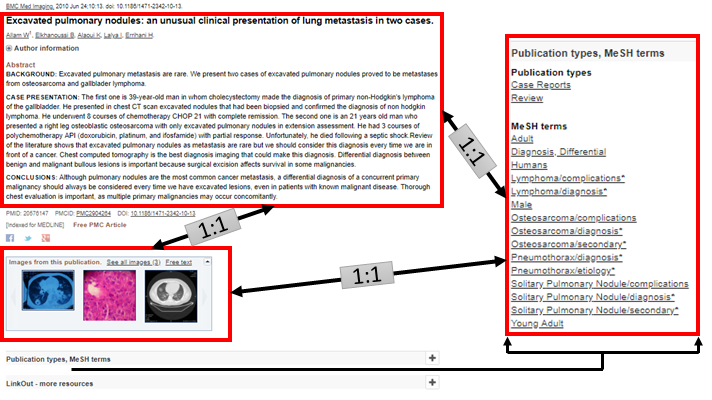
\includegraphics[height=5cm]{one_one_associationPubMed.png}
   \end{tabular}
   \end{center}
   \caption[example] 
%>>>> use \label inside caption to get Fig. number with \ref{}
   { \label{figure:1_1association} 
A typical Medline record explaining 1:1 association between the journal publication images, the full-text of the article and the manually-annotated MeSH controlled vocabulary.}
\end{figure} 
\vspace{5mm}
%
%
\subsection{Image classification with convolutional neural networks}
%
% Deep learning and CNNs
In the past few years, deep learning approaches have outperformed classical machine-learning algorithms in the analysis of histopathology images~\cite{JOA2017}
Unlike methods based on hand-crafted features, deep learning approaches build increasingly abstract representations of the data, which are learned in a hierarchical fashion.
Moreover, convolutional neural networks (CNN), a commonly used deep learning architecture for image analysis, have shown promising results in the supervised and unsupervised automatic classification of light microscopy images~\cite{JAO2017}.

% Vincent's visual classification
As an initial step in this work, a DenseNet-169 convolutional neural network, was used to generate a primary modality classification of all the images contained in the PMC-OA journal articles~\cite{HLW2017}.
The approach classified all of the PMC-OA visual data elements into 31 image modality types from the ImageCLEF 2018 challenge~\cite{IMV2018}.
It was additionally designated as a reference method for the classification of the participants data set.
The classes include modalities of diagnostic images (\emph{e.g.} DMLI, ultrasound and computed tomography), types of generic biomedical illustrations (\emph{e.g.} tables and flowcharts) and compound figures (images consisting of several sub figures). 
The network originally pre-trained on ImageNet was fine-tuned with an Adam optimizer and enhanced with data augmentation for this task. 
For more details on the implementation and training setup, refer to the visual analysis section in the original paper~\cite{AnM2018}.
Each individual DMLI classified by the network in this step, was then linked to its respective Medline record from PMC-OA using the unique PMCID.
In Fig.~\ref{fig:DMLI_samples}, some samples visually classified by this approach as DMLI are shown.
% Visual classification with VGG19
In this work, a CNN was evaluated in each of the 3 classification tasks selected to refine the curation of DMLI, similar to the initial modality classification approach.
We fine-tuned a VGG19 network for each of the classification tasks, required to obtain only rare cancer studies, both with and without data augmentation~\cite{SiZ2014}.
%
\begin{figure}
    \centering
    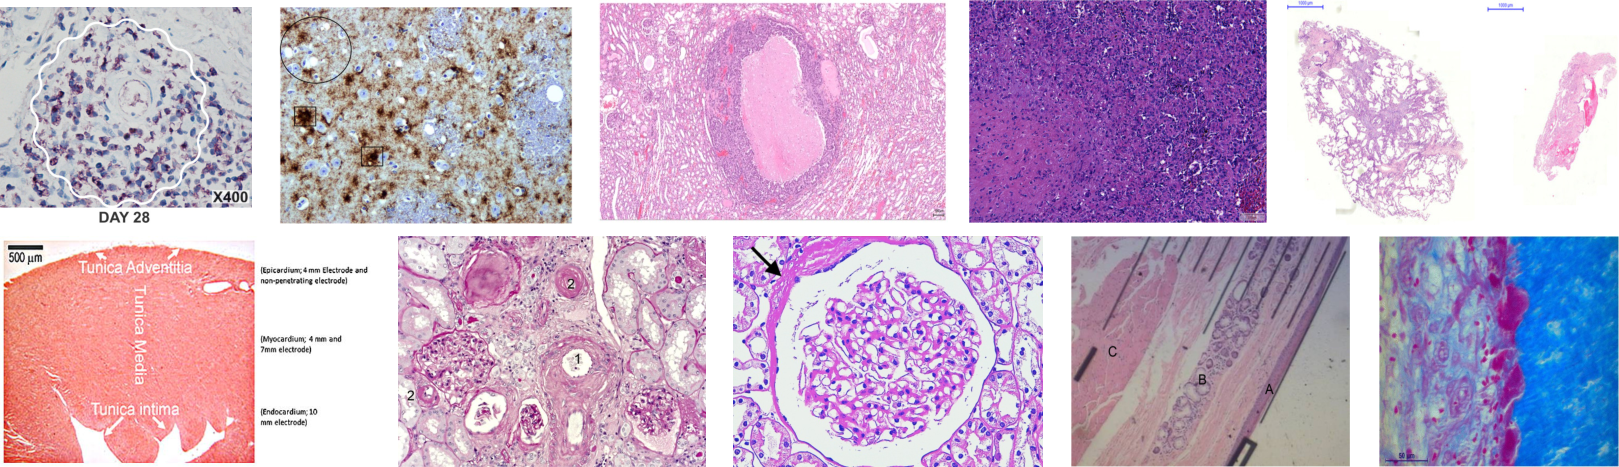
\includegraphics[width=\textwidth]{figures/samples.pdf}
    \caption{Sample images from the PMC-OA data set classified as DMLI by the reference method from the ImageCLEF 2018 challenge.}
    \label{fig:DMLI_samples}
\end{figure}
\vspace{5mm}
%
\subsection{Textual data preprocessing}
\label{subsec:text_preprocess}
%
To compare the performance of the visual classification to text, different machine learning approaches were developed relying on the full-text of the journal articles and the manually-annotated MeSH terms, when available. 
Textual data requires a thorough preprocessing before it can be utilized for any kind of extrinsic natural language processing task.
Therefore, all the Medline text records were first lowercased before being tokenized into words by NLTK\footnote{https://www.nltk.org/api/nltk.tokenize.html}.
The most frequent and noisy tokens were removed using a set of predefined stop words provided by NLTK together with specific stop words from PubMed\footnote{https://www.ncbi.nlm.nih.gov/books/NBK3827/table/pubmedhelp.T.stopwords/}. 
Additional corpus specific stop words were identified during the experiments and removed accordingly (refer Table~\ref{tab:stopwords}). 
Then a process of text normalization converted British English terms into American English. 
Lemmatization was performed using the word net lemmatizer~\cite{pmid22464129}.
A corpus vocabulary was constructed from all the unique corpus tokens. 
To scale this vocabulary down, uninformative short tokens with fewer than 3 characters and also the tokens with vocabulary count lower than five were removed assuming they were not representative of the classes.
%
\begin{table}[ht]
\caption{List of corpus-specific stop-words}
\label{tab:stopwords}
    \centering
    \begin{tabular}{|c|c|c|c|}
    \hline
        introduction & abstract & background & method(s) \\
    \hline
        materials & objective(s) & aim(d) & outcome(s) \\
    \hline
        conclusion(s) & associated & disease & induced \\
    \hline
        also & may & level(s) & show \\
    \hline
    \end{tabular}
\end{table}
%
\subsection{Text representation}
\label{subsec:textrep}
%
Proper representation of text is critical when classifying documents using machine learning (ML) methods.
Text representation methods convert text documents into a mathematical form or numeric vector understood by ML systems.
To convert the preprocessed texts from each Medline record into a numeric vector, three different methods for text representation were tested: 1) count-based vectors, 2) word vectors and 3) paragraph vectors. 

\paragraph{Count-based representation: }
One of the earliest count-based representations include bag-of-words (BoW) representation which involves representing a document by word counts for the words in the document.
Term Frequency - Inverse Document Frequency (TF-IDF) is a type of weighted, count-based method for vectorized text representation.
It is a traditional, sparse representation of text, but is also a very competitive baseline.~\cite{tfidfBow}
TF-IDF is defined by term frequency (TF) multiplied by inverse document frequency (IDF).
%\begin{math} tfidf_{i,d} = tf_{i,d} \cdot idf_{i} \end{math}
Term frequency of a word W is defined as the word count of W for the document D divided by the number of words N in D.
IDF of a word W is defined as logarithm of the total number of documents divided by the number of documents containing W.
This increases weight for the meaningful words in the corpus and reduces the weight for frequently occurring stop-words like a, an, the, in, if, of, etc.

\paragraph{Word vectors: }
Word2vec and Global Vectors for Word Representation (GloVe), also called as word embeddings, are the two unsupervised algorithms for extraction of dense, semantic, real-valued vectors from words based on their context.
While word2vec is a predictive model, GloVe is a count-based model that takes into account word co-occurrence matrix for generation of vectors. 
Both the methods capture word semantics unlike tf-idf.
In the semantic space of a word embedding, vectors for two similar words will be located near each other and have a high cosine similarity.
For example, the cosine similarity for word2vec google news model between the terms ``woman'' and ``patient'' is 0.7299, while for the terms ``mouse'' and ``patient'' is 0.3211.
For this work, three pretrained word2vec embeddings, one pre-trained GloVe embedding and a corpus-specific word2vec embedding (refer Table \ref{tab:wordvectors} for the details) were tested~\cite{pennington2014glove, bio2vec}.
Corpus-specific 300-dimensional word vectors were trained using word2vec algorithm implemented by Facebooks' fastText~\cite{bojanowski2017enriching}.
This work considers additive compositionality of word vectors and averages over all the word vectors in a single Medline study text to get a document-level representation.
%
\vspace{5mm}
\begin{table}[ht]
\caption{The table lists down word embeddings used in this work. 
It details about the type of embeddings, the text corpus used to train them and their two characteristic parameters: vector length and window size used to train the embeddings.}
\label{tab:wordvectors}
    \centering
    \begin{tabular}{|c|c|c|}
    \hline
        Embedding name & Corpus & length and window size (WS)  \\
    \hline
        word2vec & Google news & 300-dimensional \\
        bio2vec & PubMed & 300-dimensional, WS 2\\
        bio2vec & PubMed & 300-dimensional, WS 30\\
        GloVe & Wikipedia 2014, English Gigaword & 200-dimensional, WS 6\\
        word2vec & Corpus-specific & 300-dimensional, WS 5\\
    \hline
    \end{tabular}
\end{table}
\vspace{5mm}
%
\paragraph{Paragraph vectors: }
Paragraph vectors are generated in an unsupervised manner and learn distributed representation for pieces of text rather than for the individual words.
Paragraph vectors learn to associate words with document labels rather than with the other words in context.
This work used two kinds of paragraph vectors: 1) distributed memory model of paragraph vectors (PV-DM) and
2) distributed bag of words model of paragraph vectors (PV-DBOW)~\cite{le2014distributed}.
% 
\subsection{Ontology-assisted text classification}
\label{subsec:onto_classi}
%
All the MeSH-labelled text records were exploited to serially train and evaluate multiple classifiers (Logistic Regression (LR), Support Vector Machines (SVM) with linear kernel and K-nearest neighbour (KNN)) in order to retrieve human rare cancer publications. 
At each step, the classifier performance was evaluated on an independent validation set with the corresponding MeSH terms regarded as the ground truth.
GridSearch was used to identify the best text representation, best model and model parameters.
Only the setups with the best F1-scores on an unseen validation set were then used to classify the unlabelled text data (without manual MeSH terms).
%
\section{Experimental setup}
\label{subsec:pipeline}
%
\subsection{Mining out ``human" images} 
\label{subsubsec:step2}
%
All the Medline records with visual data elements initially classified as DMLI were divided into two groups corresponding to the availability of manually-attached MeSH terms.
The records with MeSH terms, considered as ground truth in this work, were further divided and labelled with three mutually-exclusive labels (``human", ``non-human" and ``ambiguous").
Any Medline record was labelled ``human'' if and only if (iff) the corresponding MeSH terms list contained MeSH code for human\footnote{https://meshb.nlm.nih.gov/record/ui?ui=D006801} (B01.050.150.900.649.313.988.400.112.400.400) and no other organism code from B01 tree-branch.
A record was labelled ``ambiguous'' iff MeSH terms contained MeSH code for human, but also for other organism code from B01 tree-branch, for example, mice\footnote{https://meshb.nlm.nih.gov/record/ui?ui=D051379} (B01.050.150.900.649.313.992.635.505.500) or rat\footnote{https://meshb.nlm.nih.gov/record/ui?ui=D051381} (B01.050.150.900.649.313.992.635.505.700).
A record was labelled ``non-human'' iff no MeSH code for human was present in the MeSH term list.
The purpose of this experiment was to precisely retrieve ``human'' instances.
As the ``ambiguous'' class records mostly represent the animal models of human tissues, this class was merged with the other instances from the class ``non-human''.

To evaluate the performance of the visual and text approaches in this classification task, the Medline records with manually-annotated MeSH terms were then divided into independent training, validation and test sets (60-20-20\%).
The training, validation and test sets used in this task were balanced accordingly to have and equal distribution of both classes in each set.
Performance measures like F1 score, Precision and Recall were tracked .

For the approaches using text in this classification task, only the title and abstract from the journal publications were considered.
% (36,770 texts)
The vectors mentioned in section \ref{subsec:textrep} were extracted from the text corpus in the training set and were used train and evaluate LR, SVM and KNN models.
Exhaustive GridSearch was used to identify the best performing text representation, model and model hyper-parameters~\cite{chicco2017ten}.
%
\setcounter{footnote}{0}
%
\subsection{Mining out ``neoplastic" images} 
\label{subsubsec:step3}
%
To obtain the records pertaining to the MeSH label ``neoplastic", the ``human" MeSH-labelled text records were divided into ``neoplastic" 
% (8,115)
and ``non-neoplastic" 
% (4,957) 
based on the presence vs. absence of the MeSH tree code (C04) covering the concept for neoplasms\footnote{https://meshb.nlm.nih.gov/record/ui?ui=D009369}. 
To account for the contribution of image captions at this stage, Medline text records were expanded to include the individual image captions emulating text augmentation.
%The new corpus with the captions included 30,550 "neoplastic" and 15,751 "non-neoplastic" instances.
This new corpus was again divided into training,  validation and test sets (60-20-20\%) for this classification task.
%This new corpus was now divided into training (37,041) and validation (9,260) sets.

In addition to the CNN visual classification of the images, two main text-based approaches were assessed. 
For the first approach, a tri-gram Bag-of-Words (BoW) model was used for feature extraction from the training set and a L2-regularized SVM was trained over it~\cite{tfidfBow}.
In the second-approach, the pre-trained 200-dimensional biomedical word embeddings were used to extract dense vectors from the training set\cite{bio2vec} and a L2-regularized SVM was then trained over these features.
Paragraph vectors PV-DM and PV-DBOW were extracted from the text records and trained on LR, SVM and KNN.
%
\subsection{Mining out ``rare cancer" images} 
\label{subsubsec:step4}
%
In this final step, all the MeSH-labelled and classified both as ``human" and ``neoplastic" text records were retained.
Since there are no manually annotated MeSH terms for ``rare cancer", a keyword-based, heuristic approach was used to extract the corresponding text records and images from ``rare cancer" studies.
This new subset was used as ground truth to estimate the performance of a convolutional neural network \emph{i.e.} VGG19 in the classification of these type of images.
%
\section{Results}
\label{sec:results}
% In the results section also show the word cloud for annotated and classified texts.
%
% DMLI - visual classification
The initial modality classification approach using visual deep learning features classified 241,728 images as ``DMLI".
Exploiting the 1:1 association (ref section \ref{subsec:dataset}), all the Medline text records (64,640) and the available MeSH terms corresponding to these ``DMLI" images were selected.
Out of these, a total of 31,733 Medline text records had manually-attached MeSH terms and 32,907 were unlabelled.

% Task 1: Human images 
Tables~\ref{table:1} and \ref{table:2} report the classification performance scores on the corresponding test sets for the ``human" (see section \ref{subsubsec:step2}) and ``neoplastic" (see section \ref{subsubsec:step3}) tasks. 
The best text-based approaches at each classification step (in bold) reach above 90\% for the precision and the recall scores. 
For the ``human" identification step, the tf-idf bi-gram representation with LR reached a 90\% mean-F1 score. 
Therefore, the tf-idf tri-grams with L2-regularized SVM model was selected as the reference method to classify the unlabelled Medline records into ``human'' and ``non-human''~\cite{le2014distributed}.


As a result of this classification step, a total of 77,746 Medline text records corresponding to the ``human" class were identified.
\vspace{5mm}
%%%%%%%%%%%%%%%%%%%%%%%%%%%%%%
% Table Human task
%%%%%%%%%%%%%%%%%%%%%%%%%%%%%%
%\FloatBarrier
\begin{table}[!htbp]
\caption{Summary and assessment for best visual and text classifier-feature combinations for the ``human" classification task, described in Section~\ref{subsubsec:step2}}
\label{table:1}
\centering
\begin{tabular}{ |p{1.5cm}|p{3.0cm}|p{5.0cm}|p{1.5cm}|p{1.5cm}|p{1.5cm}|  }
 \hline
 \multicolumn{6}{|c|}{human vs. non-human classification} \\
 \hline
 Classifier & Feature type & Feature Settings & Precision & Recall & F1\\
 \hline
\multicolumn{6}{|c|}{Visual classification} \\
\hline
VGG19 & deep learning & no data augmentation & 0.68 & 0.67 & 0.67 \\
VGG19 & deep learning & with data augmentation & 0.69 & 0.71 & 0.68 \\
\hline
\multicolumn{6}{|c|}{Text classification} \\
\hline
\textbf{SVM}   & \textbf{count-based} & \textbf{tf-idf tri-grams}    & \textbf{0.89} &  \textbf{0.90} &   \textbf{0.90} \\
 SVM & word vectors &   Corpus-specific embeddings  & 0.88   & 0.89 &   0.89\\
 LR & paragraph vectors & pvdbow (100, 30, 2) & 0.87 & 0.89 & 0.88 \\
 \hline
 \end{tabular}
\end{table}
\vspace{5mm}
%
\begin{figure}%
    \centering
    \subfloat{{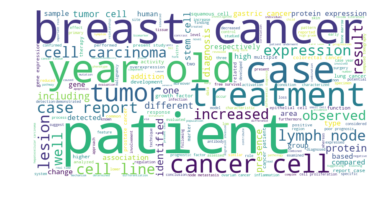
\includegraphics[width=8.1cm]{figures/human_MESH_wordcloud.png} }}
    %\qquad
    \subfloat{{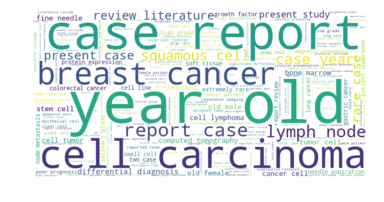
\includegraphics[width=8.1cm]{figures/human_predicted_wordcloud.png} }}
    \caption{WordCloud for the top 100 most frequent words in Medline records labelled ``human'' vs. the Medline records predicted ``human'' by the experiment in section \ref{subsubsec:step2}}%
    \label{fig:wordcloud_human}
\end{figure}
\vspace{5mm}
%
\begin{figure}%
    \centering
    \subfloat{{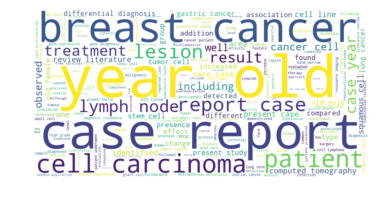
\includegraphics[width=8.1cm]{figures/human_all_wordcloud.png} }}
    %\qquad
    \subfloat{{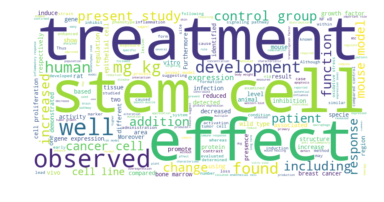
\includegraphics[width=8.1cm]{figures/animal_all_wordcloud.png} }}
    \caption{WordCloud for top 100 words most frequent tokens in Medline records labelled ``human'' vs. the Medline records predicted ``non-human''}%
    \label{fig:wordcloud_human}
\end{figure}
\vspace{5mm}
%
% Task 2: Neoplastic images
For the DMLI ``neoplastic" image identification, the top two approaches reached a mean-F1 close to a perfect classification, with the tf-idf-tri-grams being slightly better at identifying ``neoplastic" publications.
When compared to the VGG19 deep learning model, relying on visual features from the images, the top text approaches obtained a much higher precision and better recall as well (see Table ~\ref{table:2}). 
As a result of the ``neoplastic" vs. ``non-neoplastic" classification, a total of 72,551 Medline text records corresponding to the ``neoplastic" class were identified.
\vspace{5mm}
%%%%%%%%%%%%%%%%%%%%%%%%%%%%%%
% Table Neoplasm task
%%%%%%%%%%%%%%%%%%%%%%%%%%%%%%
\begin{table}[ht]
\caption{Summary and assessment for best visual and text classifier-feature combinations for the ``neoplastic" classification task, described in Section~\ref{subsubsec:step3} and its comparison to the visual classification}
\label{table:2}
\centering
\begin{tabular}{ |p{1.5cm}|p{3.0cm}|p{5.0cm}|p{1.5cm}|p{1.5cm}|p{1.5cm}|  }
 \hline
 \multicolumn{6}{|c|}{neoplastic vs. non-neoplastic classification} \\
 \hline
 Classifier  & Feature type & Features & Precision & Recall & F1\\
 \hline
\multicolumn{6}{|c|}{Visual classification} \\
\hline
VGG19 & deep learning & no data augmentation & 0.64 & 0.61 & 0.63 \\
VGG19 & deep learning & with data augmentation & 0.68 & 0.65 & 0.64 \\
\hline
\multicolumn{6}{|c|}{Text classification} \\
\hline
\textbf{SVM} & \textbf{count-based}   & \textbf{tf-idf bi-grams}    & \textbf{0.99} &  \textbf{0.99} &   \textbf{0.99} \\
 SVM & word vectors  &  Pretrained bio\_NLP vectors  & 0.98 &  0.94 &   0.96\\
 LR & paragraph vectors  & PV-DBOW & 0.98 & 0.98 & 0.98 \\
 \hline
 \end{tabular}
\end{table}
\vspace{5mm}
%
\begin{figure}%
    \centering
    \subfloat{{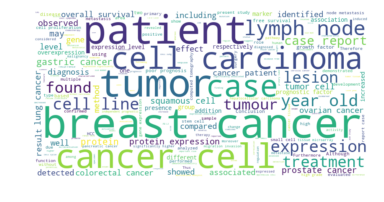
\includegraphics[width=8.1cm]{figures/word_neoplasm_MeSH.png} }}
    %\qquad
    \subfloat{{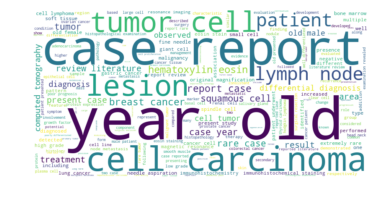
\includegraphics[width=8.1cm]{figures/word_neoplasm_predicted.png} }}
    \caption{WordCloud for the top 100 most frequent words in Medline records labelled ``neoplastic'' vs. the Medline records predicted ``neoplastic'' by the experiment in section \ref{subsubsec:step3}}%
    \label{fig:wordcloud_neoplasm}
\end{figure}
\vspace{5mm}
%
% Task 3: Rare cancer images - keyword selection
The setup with best F1-score from the two previous classification tasks was used to classify the remaining Medline text records with no manually-attached MeSH terms.
By applying a keyword-based filtering to the classified data set, 32,486 light microscopy human rare cancer open-access images were identified together with their corresponding journal articles contaning highly-correlated text information. 
The visual classification for this final task, using deep learning features with data augmentation, resulted in an F1-score of 0.71.
%and a set of 20,553 images that correspond to human cancer but are not rare.
%
%%%%%%%%%%%%%%%%%%%%%%%%%%%%%%
% Table Rare cancer task
%%%%%%%%%%%%%%%%%%%%%%%%%%%%%%
\begin{table}[ht]
\caption{Summary and assessment for the visual classification of ``rare cancer" vs. ``non-rare cancer" images.}
\label{table:3}
\centering
\begin{tabular}{ |p{1.5cm}|p{3.0cm}|p{5.0cm}|p{1.5cm}|p{1.5cm}|p{1.5cm}|  }
 \hline
 \multicolumn{6}{|c|}{rare cancer vs. non-rare cancer classification} \\
 \hline
 Classifier  & Feature type & Features & Precision & Recall & F1\\
 \hline
\multicolumn{6}{|c|}{Visual classification} \\
\hline
VGG19 & deep learning & no data augmentation & 0.68 & 0.66 & 0.67 \\
\textbf{VGG19} & \textbf{deep learning} & \textbf{with data augmentation} & \textbf{0.71} & \textbf{0.66} & \textbf{0.68} \\
\hline
 \end{tabular}
\end{table}
\vspace{5mm}
%
\section{Discussion}
%
To the best of our knowledge this is the first study targeting the automatic curation of rare cancer images in journal publications from the biomedical literature.
The proposed approach relied on both the visual and text information from the freely available publications in the PMC-OA repository.
The final pipeline contained the following steps: 1) mining out ``DMLI" images, 2) mining out ``human" images, 3) mining out ``neoplastic" (tumor-related) images, and finally 4) mining out human ``rare cancer" light microscopy images with their corresponding journal articles.

% - Human v nonHuman (conclusions)
When comparing the textual vs. visual classification performance in both the ``human'' vs. ``non-human" task, and the ``neoplastic" vs. ``non-neoplastic" task, textual features performed considerably better compared to the visual features.
The the BoW tri-gram approach with an SVM classifier was the best approach for both tasks, relying on count-based features.
Nevertheless, visual features could correctly classify some test images with a recall score of up to 0.71 in the ``human" identification task.
It is important to note that the class ``ambiguous'' was merged with the class ``non-human'', thus influencing the classification results for both visual and textual features.
For the ``neoplastic'' vs. ``non-neoplastic'' classification, the visual features gave a worse performance with a maximum F1 score of 0.64.
The results are slightly better for the visual approaches in the ``rare cancer" vs. ``non-rare cancer" task, but still there is room for improvement. 
Some of the images and diseases that have been identified in this pipeline are shown in Fig.~\ref{fig:rare_cancers}.

In this work, we compared the advantages and limitations of the visual classification of the images vs. the text classification of some text elements from the corresponding journal publications (title, abstract). 
The results show that with the current number of images available, the simpler and more interpretable text mining approaches (tf-idf) outperform state-of-the-art visual strategies. 
However, it is important to consider that the classification performed on the individual images from a publication is not on the same level as the classification of the full-text. 
With the combination of an initial DMLI classification based only on the visual features, and the subsequent text mining non light microscopy images were excluded from the final data set.
The PubMed Central Open Access repository includes more than 2.09 million publications and is continuously being updated with novel full-text biomedical scientific publications, including the latest rare cancer studies.
Since the PMC-OA data set will continue to grow in the following years, this is an initial framework to automatically generate high-quality biomedical and multimodal data sets that could potentially improve the understanding of these type of diseases.
% future work
Our future research direction is towards experimenting with the multimodal fusion of visual and textual representations from individual images and journal articles~\cite{arevalo2017gated}.
%
%https://www.overleaf.com/project/5da7227d6197540001d0956a
\begin{figure}
    \centering
    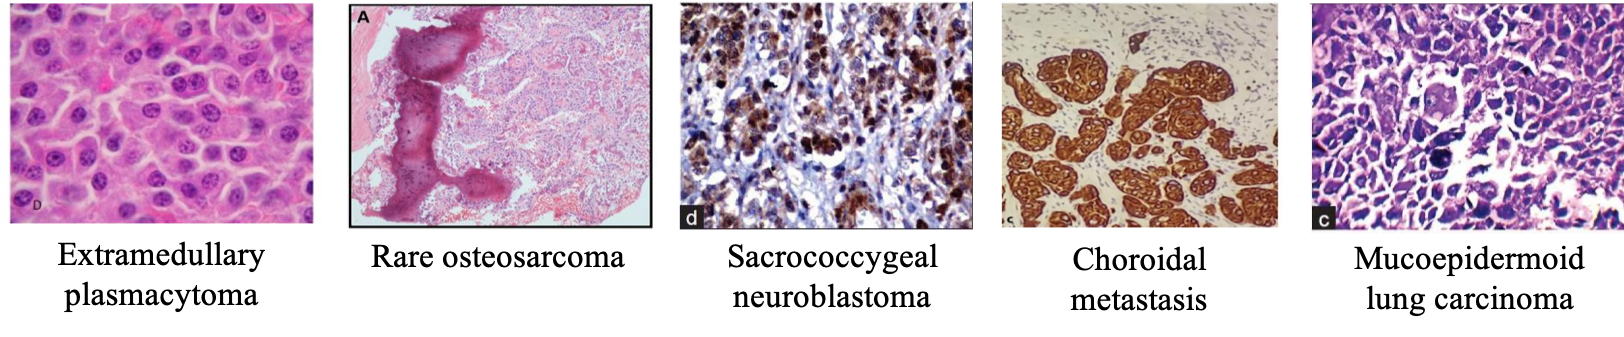
\includegraphics[width=\textwidth]{figures/samples_predicted_rareCancers.png}
    \caption{Sample light microscopy human rare cancer images mined out with the proposed approach. Some of the samples come from PMC-OA publications with no MeSH terms available.}
    \label{fig:rare_cancers}
\end{figure}
\vspace{5mm}
%
%
\section{Conclusions}
%
In this work we present a framework, using visual deep learning and natural language processing methods, to mine out 32,486 light microscopy human rare cancer images. 
The generated multimodal dataset can fill the void of information regarding the study of these diseases and be further used by researchers as an automatically annotated data base for the development of new clinical models.
A more comprehensive understanding of the changes present in these cancers, could potentially help to improve the outcome of these patients. 
%
\acknowledgments % equivalent to \section*{ACKNOWLEDGMENTS}
%
This work was partially funded by the EU in the context of the H2020 project ExaMode.
%
% References
\bibliography{report} % bibliography data in report.bib
\bibliographystyle{spiebib} % makes bibtex use spiebib.bst
%
\end{document} 